\subsubsection*{Определение параметров для \na}
\vspace{-5mm}

\begin{figure}[h!]
    \centering
    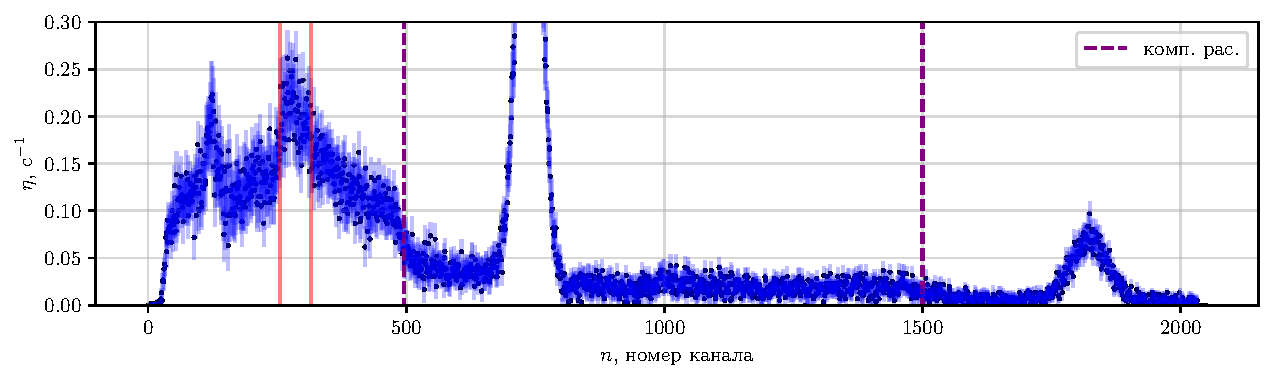
\includegraphics[width=0.95\textwidth]{figures/na_0.pdf}
    % \vspace{-2mm}
    % \caption{Общий вид спектра \cs}
    %\label{fig:}
\end{figure}

\vspace{-5mm}

\begin{figure}[h!]
    \centering
    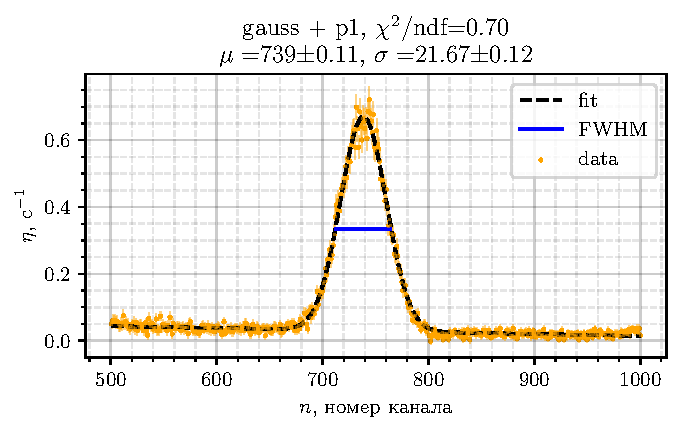
\includegraphics[width=0.49\textwidth]{figures/na_p1.pdf}
    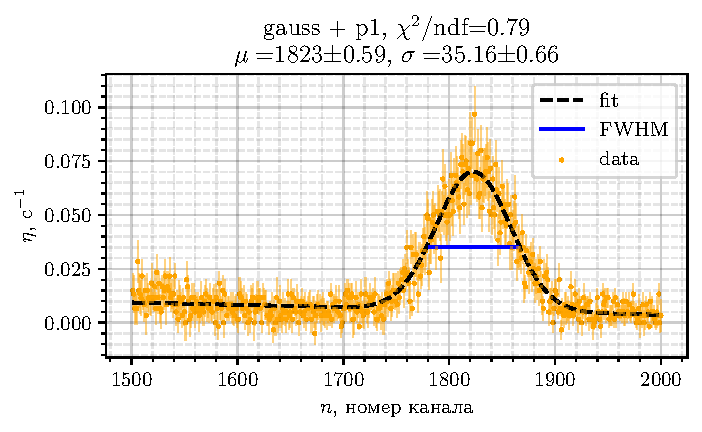
\includegraphics[width=0.49\textwidth]{figures/na_p2.pdf}
    \vspace{-2mm}
    \caption{Определение параметров пиков полного поглощения \na}
    %\label{fig:}
\end{figure}

\vspace{-5mm}

\begin{figure}[h!]
    \centering
    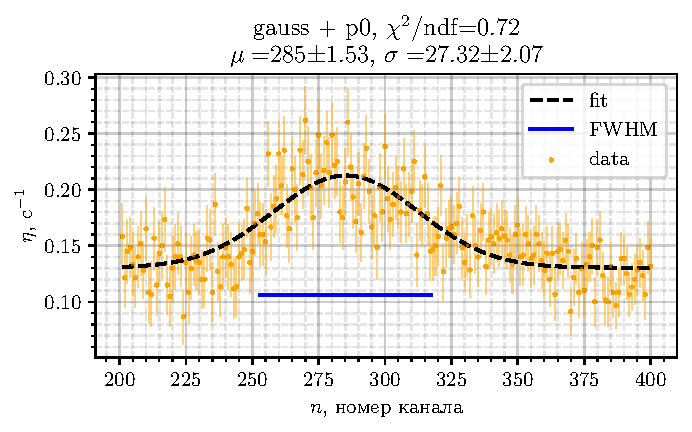
\includegraphics[width=0.5\textwidth]{figures/na_bp1.pdf}
    \\
    \vspace{-2mm}
    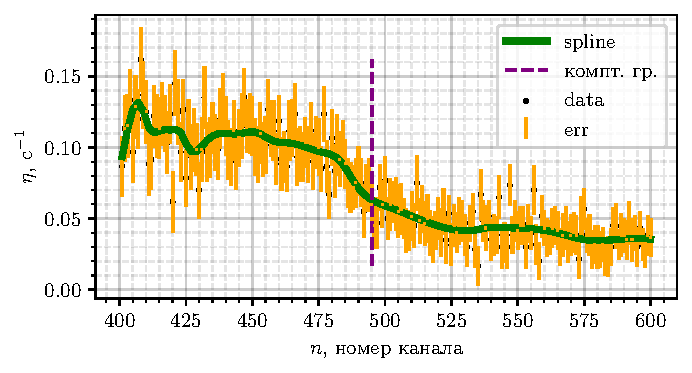
\includegraphics[width=0.49\textwidth]{figures/na_comp1.pdf}
    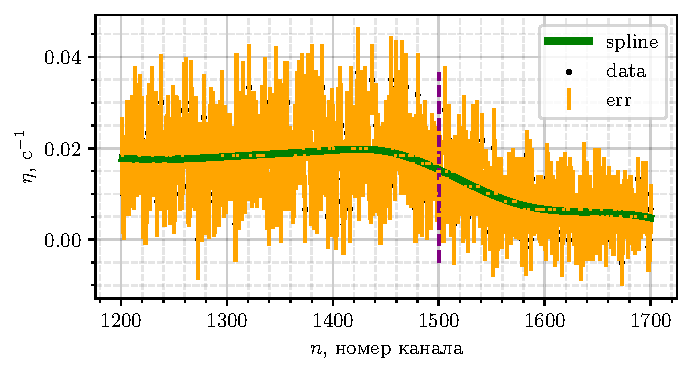
\includegraphics[width=0.49\textwidth]{figures/na_comp2.pdf}
    \vspace{-2mm}
    \caption{Определение края комптоновского рассеяния и пика обратного рассеяния для \na}
\end{figure}

\newpage


\subsubsection*{Определение параметров для \cs}
% \vspace{-5mm}

\begin{figure}[h!]
    \centering
    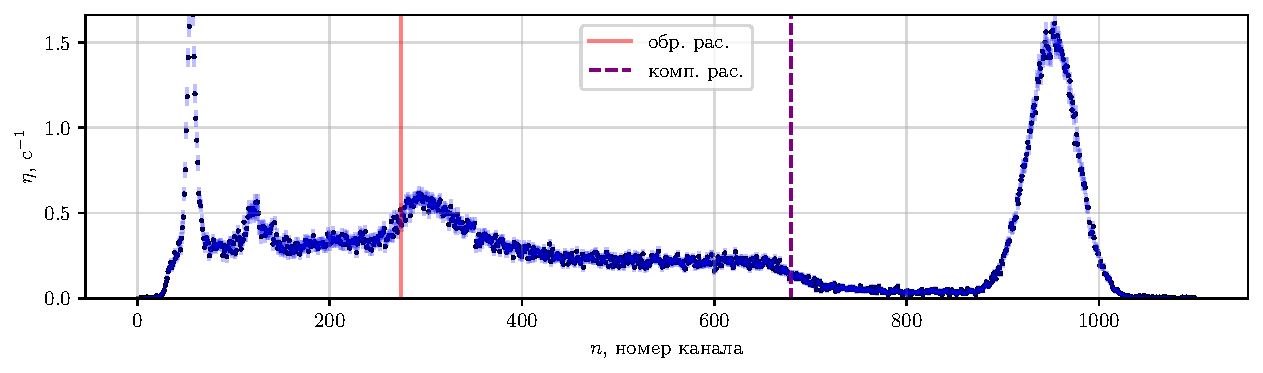
\includegraphics[width=0.95\textwidth]{figures/cs_0.pdf}
    \vspace{-2mm}
    \caption{Общий вид спектра \cs}
    %\label{fig:}
\end{figure}



\begin{figure}[h!]
    \centering
    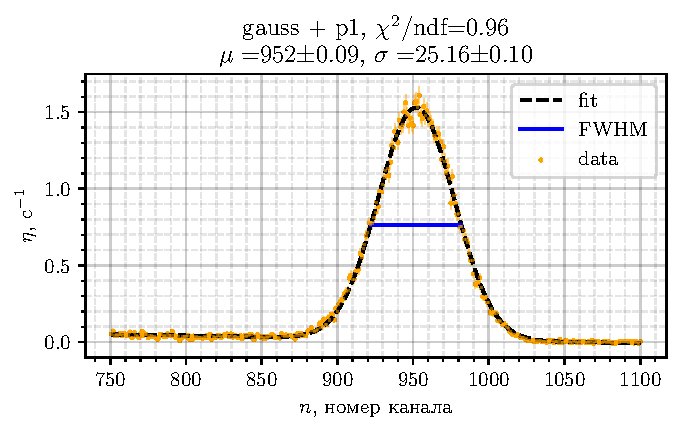
\includegraphics[width=0.49\textwidth]{figures/cs_p1.pdf}
    \vspace{-2mm}
    \caption{Определение параметров пиков полного поглощения \cs}
    %\label{fig:}
\end{figure}



\begin{figure}[h!]
    \centering
    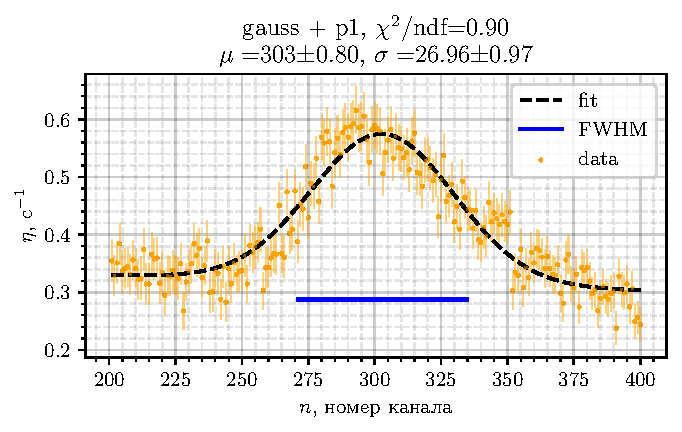
\includegraphics[width=0.49\textwidth]{figures/cs_bp1.pdf}
    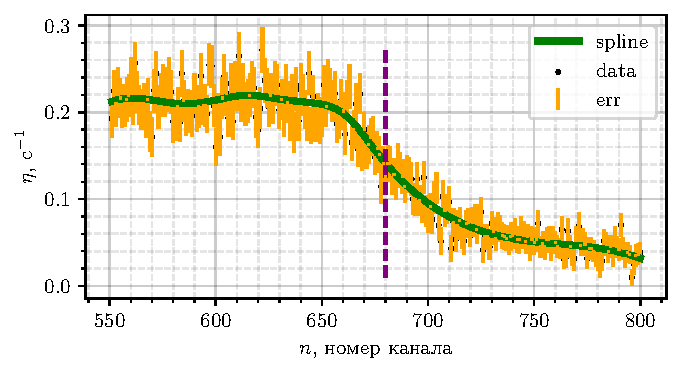
\includegraphics[width=0.49\textwidth]{figures/cs_comp1.pdf}
    \vspace{-2mm}
    \caption{Определение края комптоновского рассеяния и пика обратного рассеяния для \cs}
\end{figure}


% \newpage


% \subsubsection*{Определение параметров для \cs}


% \begin{figure}[h!]
%     \centering
%     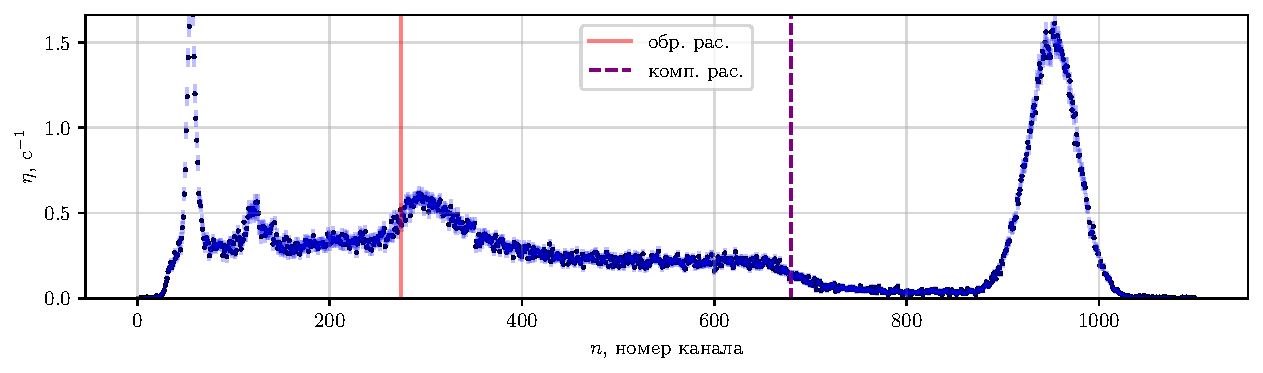
\includegraphics[width=0.95\textwidth]{figures/cs_0.pdf}
%     \vspace{-2mm}
%     \caption{Общий вид спектра \cs}
%     %\label{fig:}
% \end{figure}



% \begin{figure}[h!]
%     \centering
%     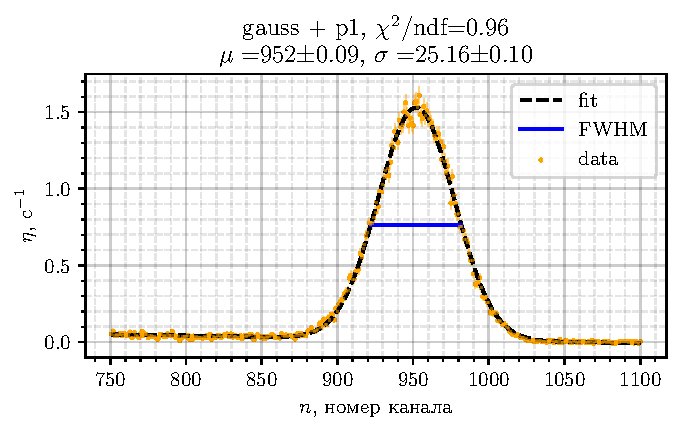
\includegraphics[width=0.49\textwidth]{figures/cs_p1.pdf}
%     \vspace{-2mm}
%     \caption{Определение параметров пиков полного поглощения \cs}
%     %\label{fig:}
% \end{figure}



% \begin{figure}[h!]
%     \centering
%     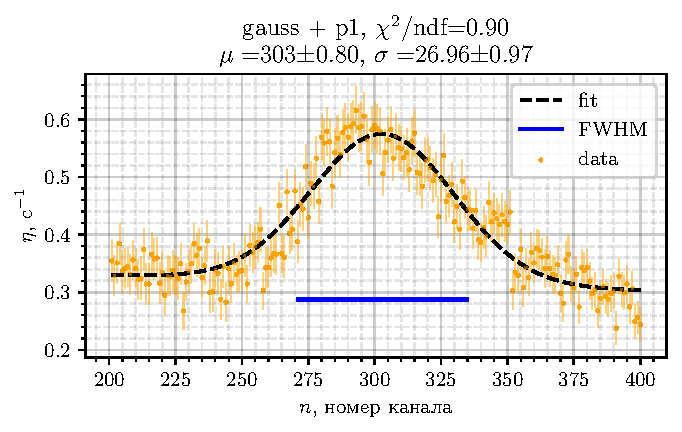
\includegraphics[width=0.49\textwidth]{figures/cs_bp1.pdf}
%     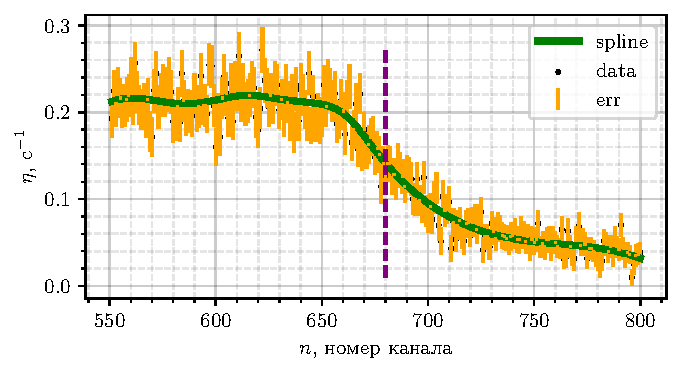
\includegraphics[width=0.49\textwidth]{figures/cs_comp1.pdf}
%     \vspace{-2mm}
%     \caption{Определение края комптоновского рассеяния и пика обратного рассеяния для \cs}
% \end{figure}



\newpage


\subsubsection*{Определение параметров для \co}


\begin{figure}[h!]
    \centering
    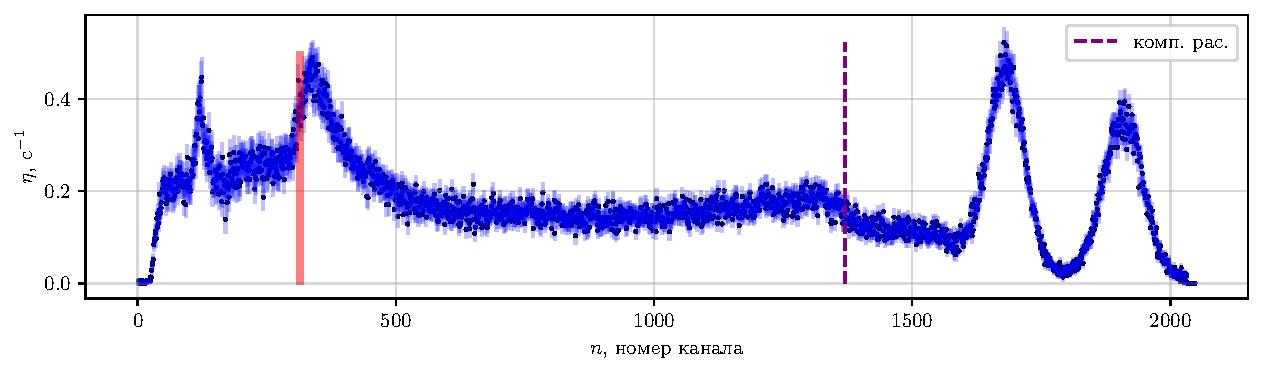
\includegraphics[width=0.95\textwidth]{figures/co_0.pdf}
    % \vspace{-2mm}
    \caption{Общий вид спектра \co}
    %\label{fig:}
\end{figure}



\begin{figure}[h!]
    \centering
    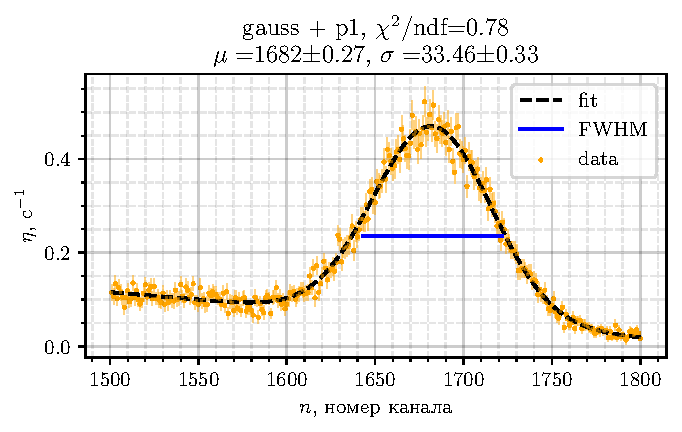
\includegraphics[width=0.49\textwidth]{figures/co_p1.pdf}
    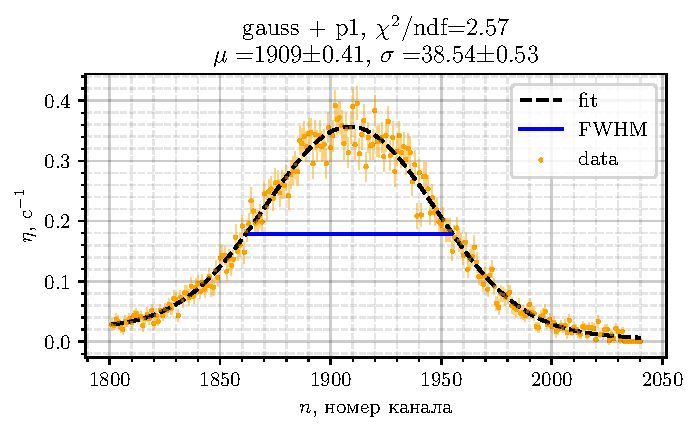
\includegraphics[width=0.49\textwidth]{figures/co_p2.pdf}
    \vspace{-2mm}
    \caption{Определение параметров пиков полного поглощения \co}
    %\label{fig:}
\end{figure}



\begin{figure}[h!]
    \centering
    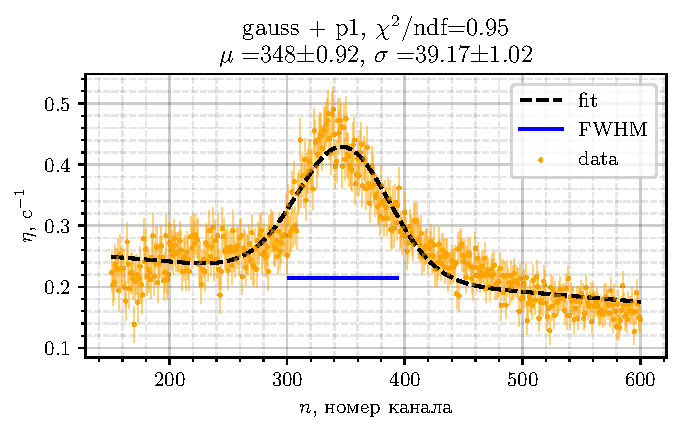
\includegraphics[width=0.5\textwidth]{figures/co_bp1.pdf}
    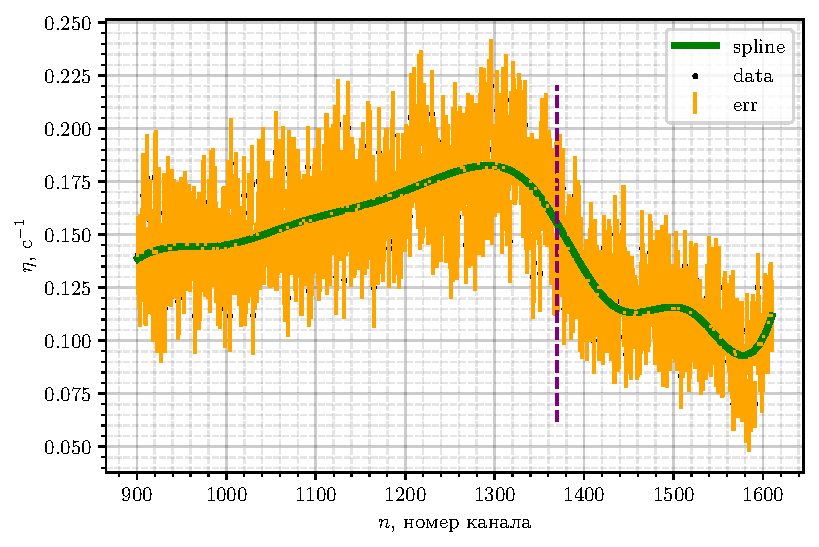
\includegraphics[width=0.49\textwidth]{figures/co_comp1.pdf}
    \vspace{-2mm}
    \caption{Определение края комптоновского рассеяния и пика обратного рассеяния для \co}
\end{figure}



\newpage


\subsubsection*{Определение параметров для \am}



\begin{figure}[h!]
    \centering
    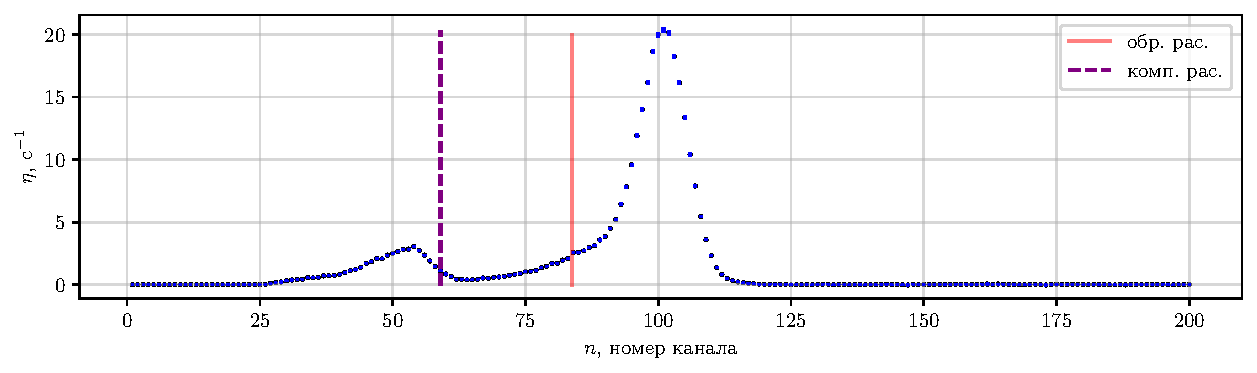
\includegraphics[width=0.95\textwidth]{figures/am_0.pdf}
    % \vspace{-2mm}
    \caption{Общий вид спектра \am}
    %\label{fig:}
\end{figure}



\begin{figure}[h!]
    \centering
    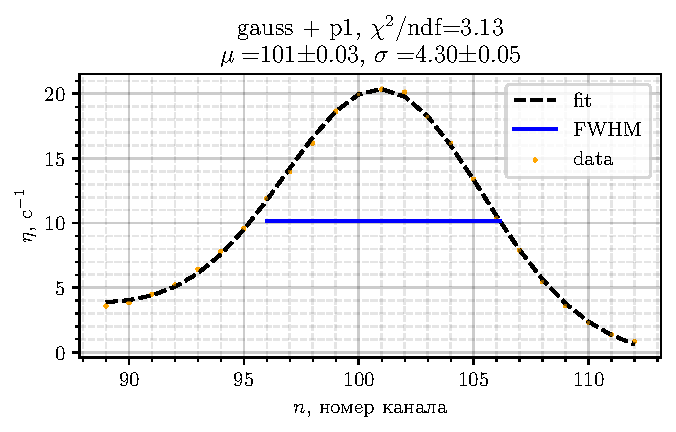
\includegraphics[width=0.49\textwidth]{figures/am_p1.pdf}
    \vspace{-2mm}
    \caption{Определение параметров пиков полного поглощения \co}
    %\label{fig:}
\end{figure}


\begin{figure}[h!]
    \centering
    % \includegraphics[width=0.5\textwidth]{figures/am_bp1.pdf}
    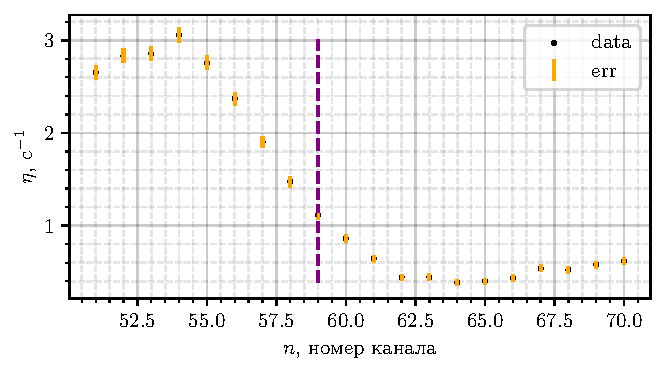
\includegraphics[width=0.49\textwidth]{figures/am_comp1.pdf}
    \vspace{-2mm}
    \caption{Определение края комптоновского рассеяния \am}
\end{figure}



\newpage

\subsubsection*{Определение параметров для \eu}
\vspace{-5mm}

\begin{figure}[h!]
    \centering
    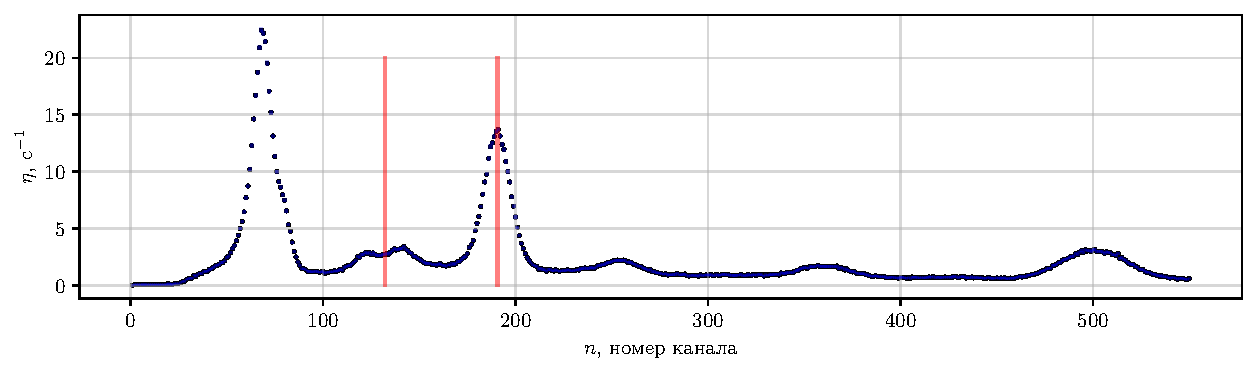
\includegraphics[width=0.95\textwidth]{figures/eu_0.pdf}
    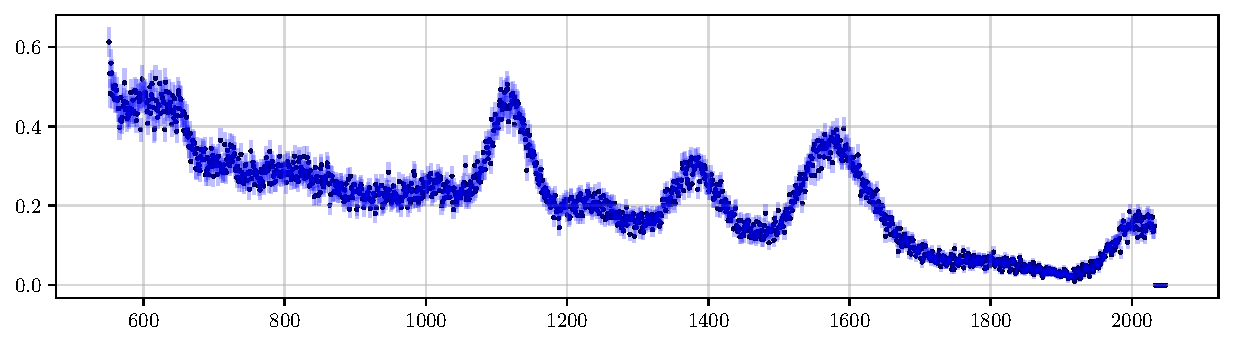
\includegraphics[width=0.95\textwidth]{figures/eu_1.pdf}
    % \vspace{-2mm}
    \caption{Общий вид спектра \cs}
    %\label{fig:}
\end{figure}

% \vspace{-5mm}

\begin{figure}[h!]
    \centering
    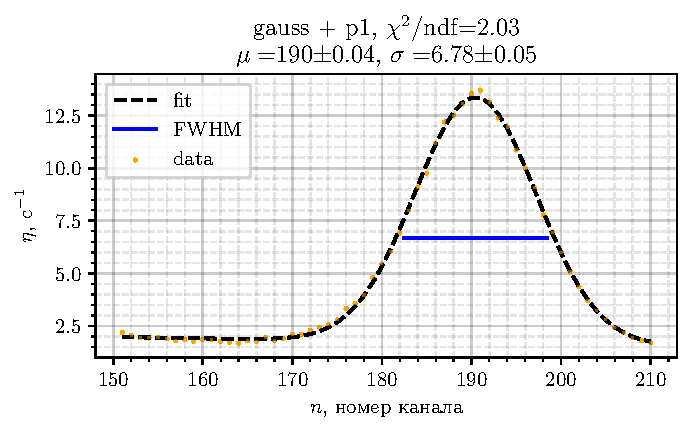
\includegraphics[width=0.49\textwidth]{figures/eu_p1.pdf}
    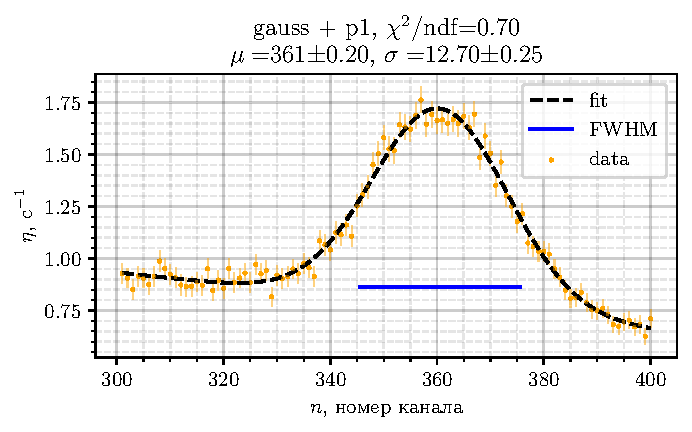
\includegraphics[width=0.49\textwidth]{figures/eu_p2.pdf} 
    \\
    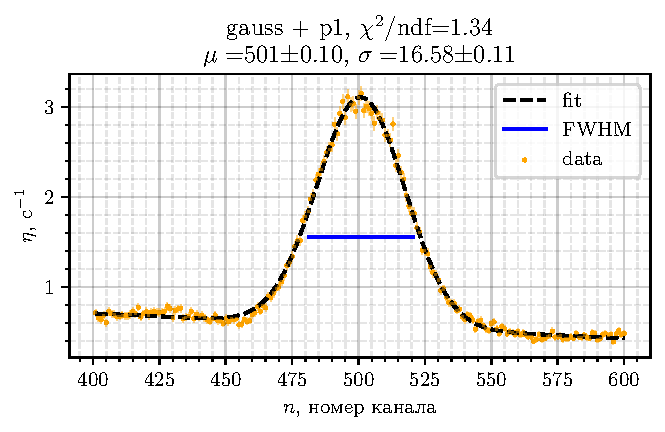
\includegraphics[width=0.49\textwidth]{figures/eu_p3.pdf}
    % 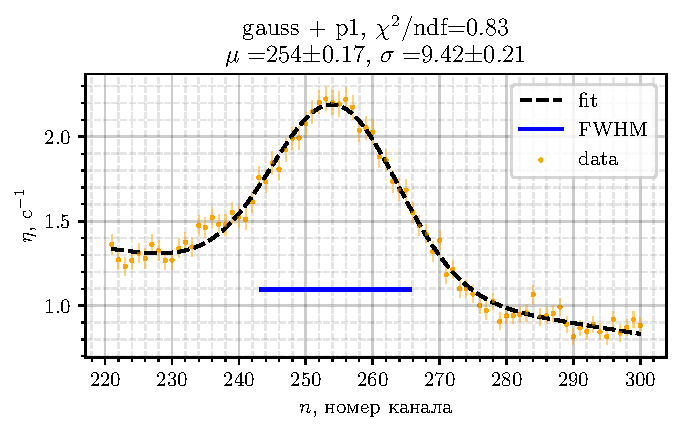
\includegraphics[width=0.5\textwidth]{figures/eu_bp1.pdf}
    \vspace{-2mm}
    \caption{Определение параметров пиков полного поглощения \eu}
    %\label{fig:}
\end{figure}

\newpage

\begin{figure}[h!]
    \centering
    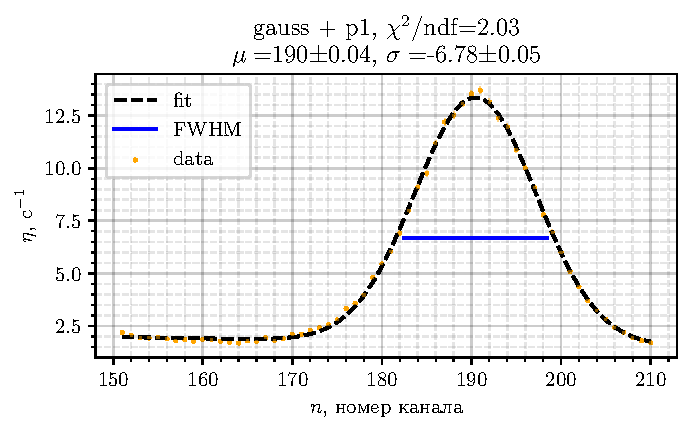
\includegraphics[width=0.5\textwidth]{figures/eu_bp2.pdf}
    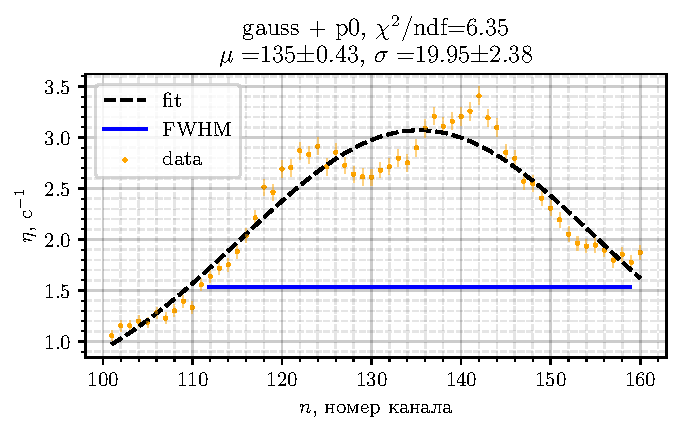
\includegraphics[width=0.49\textwidth]{figures/eu_bp3.pdf}
    \vspace{-2mm}
    \caption{Определение параметров пика обратного рассеяния для \eu}
\end{figure}

% \vspace{-5mm}

% \begin{figure}[h!]
%     \centering
%     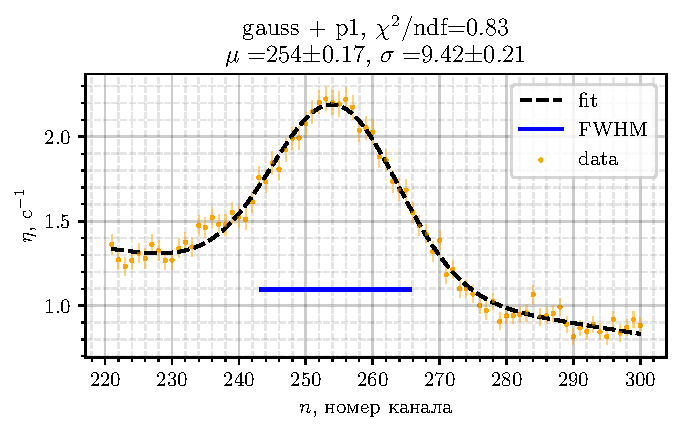
\includegraphics[width=0.5\textwidth]{figures/eu_bp1.pdf}
%     % \\
%     \vspace{-2mm}
%     % \includegraphics[width=0.49\textwidth]{figures/eu_comp1.pdf}
%     % \includegraphics[width=0.49\textwidth]{figures/eu_comp2.pdf}
%     \vspace{-2mm}
%     \caption{Определение края комптоновского рассеяния и пика обратного рассеяния для \eu}
% \end{figure}


\subsubsection*{Измерение фона}

\begin{figure}[h]
    \centering
    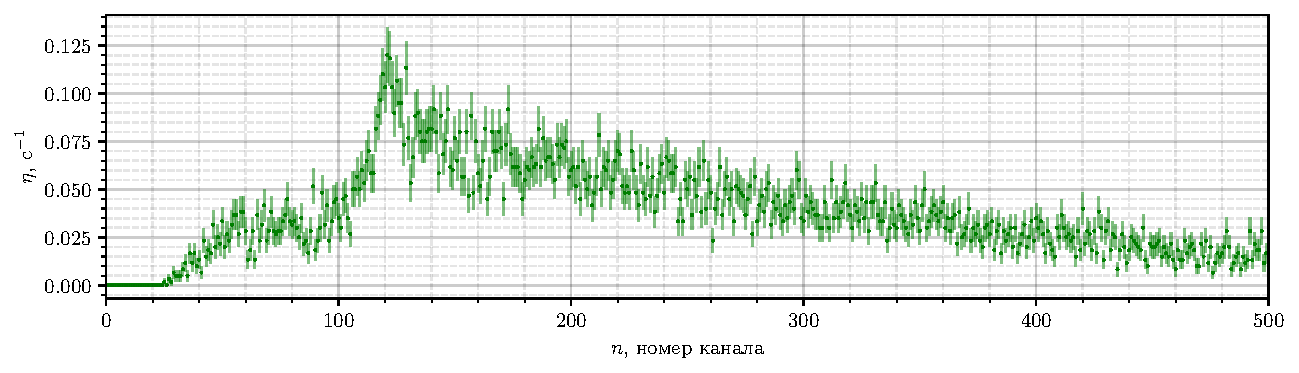
\includegraphics[width=\textwidth]{figures/bbb.pdf}
    \caption{Фоновый гамма-спектр}
    \label{fig:background}
\end{figure}
